\section{Introduction}

Explainable recommendation asks a system to predict user preferences and to
justify those predictions with natural-language explanations
\cite{explainable_rec_survey}. In cross-domain settings this problem becomes
especially fragile: evidence can transfer across domains, but review
conventions, item vocabularies, and explanation styles can shift at the same
time \cite{crossdomain_survey}. A generator that appears fluent in the target
domain may still produce explanations that are generic, repetitive, or weakly
connected to the user--item evidence. We refer to this failure mode as
explanation degeneration.

D4C provides the closest causal foundation for this problem \cite{d4c}. Its
key insight is not only that hidden textual attributes \(W\) can act as
domain-level shortcuts, but that these shortcuts participate in a dynamic
feedback process. Textual attributes at time \(t\) influence explanations, and
generated or observed explanations can reshape future textual attributes:
\[
  W^{(t)} \rightarrow E^{(t)} \rightarrow W^{(t+1)} .
\]
This dynamic view explains why degeneration can be self-reinforcing. Ordinary
generators can learn a shortcut from \(W^{(t)}\) to \(E^{(t)}\), preserving
domain-looking language while weakening the genuine user--item interaction
path that should support an explanation.

ODCR builds on this dynamic feedback diagnosis. Its starting point is that a
single coarse textual variable \(W^{(t)}\) is too broad for controlled
explanation learning. The variable mixes at least three forces: stable content
evidence, feedback-sensitive expression style, and the reliability of
counterfactual evidence. ODCR therefore refines the D4C textual-feedback view
as
\[
  W^{(t)} \Rightarrow (C, S^{(t)}, R_{cf}),
\]
where \(C\) denotes stable content evidence, \(S^{(t)}\) denotes a dynamic
hierarchical style state, and \(R_{cf}\) denotes the reliability with which
counterfactual evidence should influence learning. The resulting method is not
an engineering-stage pipeline. It is a reliability-gated dynamic causal control
framework for cross-domain explainable recommendation.

\begin{figure}[t]
  \centering
  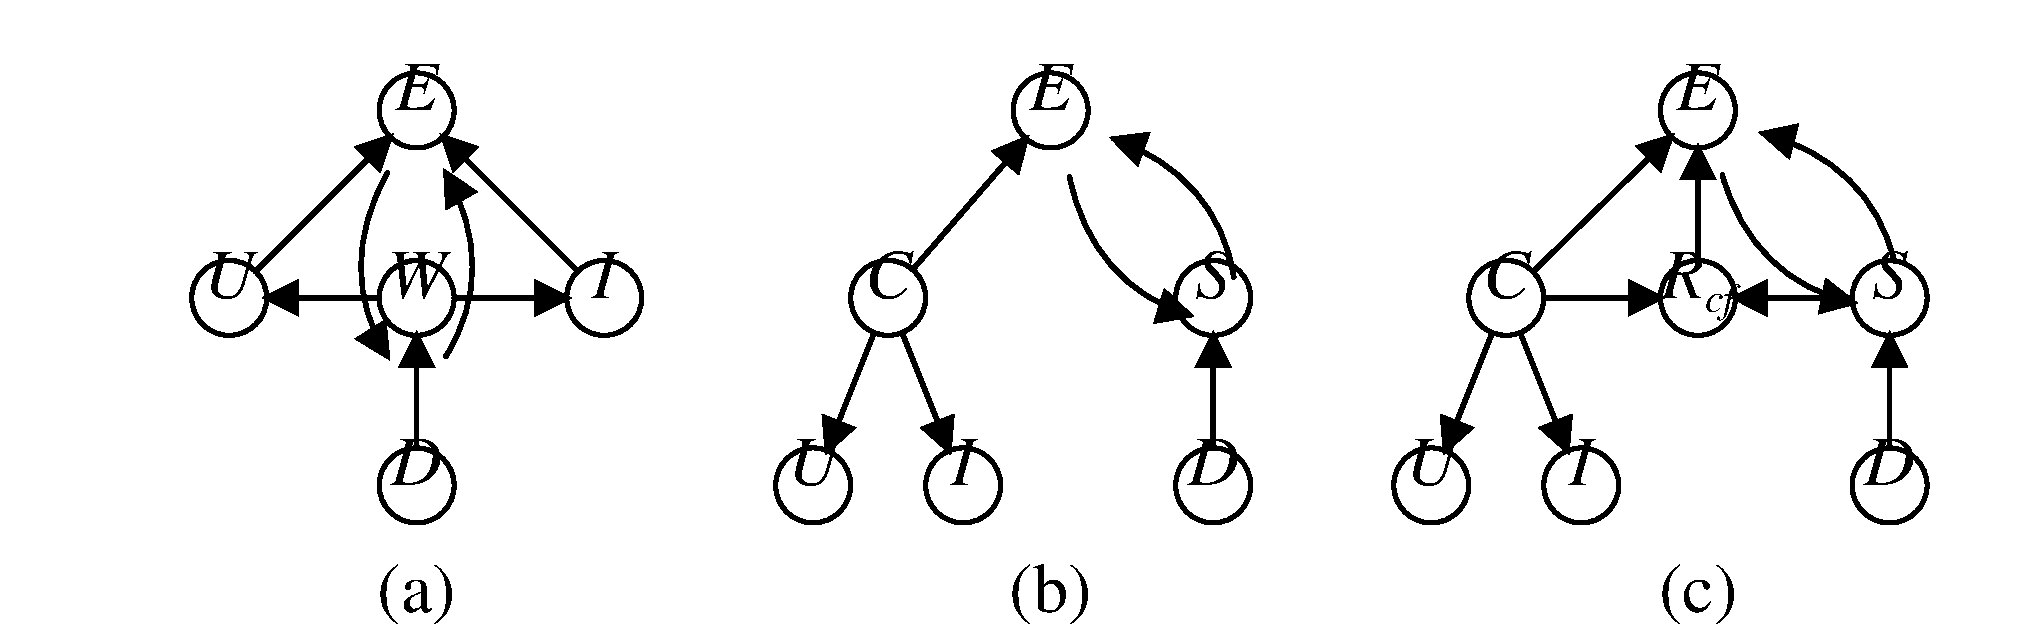
\includegraphics[width=\textwidth]{figures/figure1_dynamic_causal_refinement.pdf}
  \caption{Dynamic causal refinement from D4C to ODCR. D4C explains explanation degeneration as a feedback loop between contextual textual attributes and explanations. ODCR refines this loop into stable content evidence, feedback-sensitive hierarchical style, and counterfactual reliability control.}
  \label{fig:causal_refinement}
\end{figure}

Figure~\ref{fig:causal_refinement} summarizes the refinement. ODCR first
anchors content/style decomposition in evidence, so that content \(C\) captures
what should be explained while style \(S^{(t)}\) captures how the explanation
is expressed. It then models style hierarchically as a domain-global state plus
instance-local residual, localizing dynamic feedback to style rather than
allowing feedback to overwrite content. Counterfactual examples are further
filtered and weighted by \(R_{cf}\), so unreliable shifts do not dominate
learning. Finally, the explanation generator is conditioned on
\((U,I,C,S,R_{cf})\), with faithfulness alignment keeping generated content
consistent with rating-relevant evidence.

This manuscript makes four contributions:
\begin{itemize}
  \item \textbf{Dynamic causal refinement.} ODCR builds on D4C's dynamic
  textual-feedback diagnosis and refines coarse textual attributes into
  controllable variables for content, style, and counterfactual reliability.
  \item \textbf{Evidence-anchored decomposition.} ODCR separates stable
  content evidence from feedback-sensitive domain style, avoiding an
  undifferentiated textual shortcut.
  \item \textbf{Reliability-gated counterfactual control.} ODCR filters,
  routes, and weights counterfactual evidence using reliability and
  uncertainty-aware signals.
  \item \textbf{Controlled faithful generation.} ODCR generates explanations
  conditioned on content, style, and reliability-controlled evidence while
  keeping explanation content aligned with rating-relevant evidence.
\end{itemize}
